\documentclass[11pt,a4paper]{article}
\usepackage[latin1]{inputenc}
\usepackage[margin=1in]{geometry}
\usepackage{amsmath}
\usepackage{amsfonts}
\usepackage{amssymb}
\usepackage{graphicx}
\setlength\abovedisplayskip{0pt}
\author{James Brissette}
\title{CS-6350: HW 2}
\begin{document}
	\maketitle
	
	\section{Linear Classifiers and Boolean Functions}
		\begin{enumerate}
			\item $ $
			\item $ $
			\item $ $
			\item $ $
			\item $ $
		\end{enumerate}
	
	\section{Feature transformations}
		\begin{enumerate}
			\item 
			\item 
		\end{enumerate}
	
	\section{Mistake Bound Model of Learning}
		\begin{enumerate}
			\item $ $
			\begin{enumerate}
				\item
				\item
			\end{enumerate}
			\item A linear classifier compatible with the given data set is given by the below
			\begin{enumerate}
				\item
				\item
			\end{enumerate}
		\end{enumerate}
	
	\section{The Perceptron Algorithm and its Variants}
		\begin{enumerate}
			\item
			\item
			\item Noting that the random initialization may sometimes give different results with respect to the best hyper-parameters, in most cases I ran the 5-fold cross validation (for ten epochs each) several times and averaged them to see, on average, which parameters were actually the best. My results were as follows:\\ \\
			\textbf{Simple Perceptron}    \\
			a) rate = \{.01\}  \\
			b) cross-validation accuracy using rate=.01 was \textbf{0.612733}\\
			c) total number of updates on the training set was \textbf{6015}\\
			d) the best accuracy on the development set came with using 16 epochs and yielded an accuracy of \textbf{.735} (see below for the plot used to determine the best epoch to use). This yielded a weight vector, bias combination as follows:\\
			\begin{gather}
				w = [-4.790801  , -6.310801  , 18.629199  ,  0.809199  , -9.290801,\\
				-8.960801  , -3.480801  ,  1.899199  ,  0.75067916, -1.05087573,\\
				0.91483852,  1.0267039 ,  3.30614975,  1.8007971 ,  0.88184558,\\
				0.41990239, -2.7867524 , -0.66128905, -2.170801  ] \\
				b = -4.567802999999947
			\end{gather}
			e) using the weight vector and bias from epoch 16 to predict on the test set, the algorithm reported an accuracy of \textbf{.587065} \\
			f)
			\begin{center}
				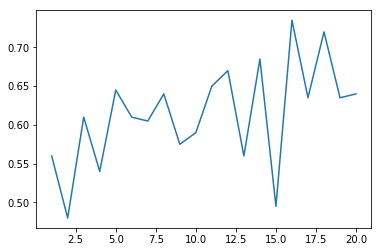
\includegraphics[width=0.7\linewidth]{simple_plot}
			\end{center}
			\\
			\textbf{Decaying Perceptron}    \\
			a) For the specific combination of the random shuffling of the training data and the initial weight vector and bias, I found the optimal initial rate = \{1\}  \\
			b) cross-validation accuracy using rate=1 was \textbf{0.664533}\\
			c) total number of updates on the training set was \textbf{5113}\\
			d) the best accuracy on the development set came with using 17 epochs and yielded an accuracy of \textbf{.71} (see below for the plot used to determine the best epoch to use). This yielded a weight vector, bias combination as follows:\\
			\begin{gather}
			w = [-0.52830582, -0.62562476,  4.58366762,  1.83460061, -0.48774808,\\
			-2.43257835, -2.71244112, -1.11330101,  0.85833871, -1.40136228,\\
			-2.3033998 , -1.70711248,  0.57267534,  0.43230634,  0.20699507,\\
			0.06603351, -0.31253566, -0.08022425, -0.59702606] \\
			b = -32.005986
			\end{gather}
			e) using the weight vector and bias from epoch 17 to predict on the test set, the algorithm reported an accuracy of \textbf{.71144} \\
			f)
			\begin{center}
				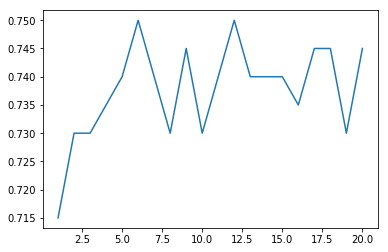
\includegraphics[width=0.7\linewidth]{decaying_plot}
			\end{center}
			\\
			\textbf{Margin Perceptron}    \\
			a) For the specific combination of the random shuffling of the training data and the initial weight vector and bias, I found the optimal combination of hyper-parameters to be margin=.01, rate=1  \\
			b) cross-validation accuracy using margin=.01, rate=1 was \textbf{0.6880}\\
			c) total number of updates on the training set was \textbf{4930}\\
			d) the best accuracy on the development set came with using 14 epochs and yielded an accuracy of \textbf{.6} (see below for the plot used to determine the best epoch to use). This yielded a weight vector, bias combination as follows:\\
			\begin{gather}
			w = [-0.54624921, -0.95548707,  2.26801139,  0.52011042, -1.45902761,\\
			-1.02471788,  0.10777735, -0.68208914, -0.01616318, -0.57514031,\\
			0.97513725,  0.30675042,  0.21458043,  0.21317788,  0.17914802,\\
			0.07836919, -0.30403893, -0.05202941,  0.01070719] \\
			b = -1.008271999999998
			\end{gather}
			e) using the weight vector and bias from epoch 14 to predict on the test set, the algorithm reported an accuracy of \textbf{.721393} \\
			f)
			\begin{center}
				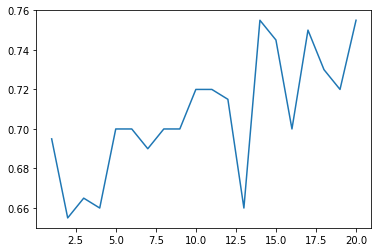
\includegraphics[width=0.7\linewidth]{margin_plot}
			\end{center}
			\item
		\end{enumerate}
	
\end{document}